\documentclass[tikz,border=6mm]{standalone}
\usepackage{amsmath,amssymb}
\usepackage{fontspec}

\usetikzlibrary{positioning,arrows.meta,shapes.geometric,fit,backgrounds,calc}

% Master Academic Palette (WCAG AA & Color-Vision Deficiency Compliant)
\definecolor{navyblue}{RGB}{30, 60, 105}    % #1E3C69 - Model architectures, encoders, primary flows
\definecolor{tealblue}{RGB}{20, 110, 105}   % #146E69 - Data plane, ingestion, datasets, gold annotations
\definecolor{purplecat}{RGB}{95, 45, 120}   % #5F2D78 - Multi-task balancing, loss dynamics, statistics
\definecolor{ambergold}{RGB}{180, 85, 15}   % #B4550F - Hardware testbed, serving trials, embeddings
\definecolor{forestgreen}{RGB}{25, 115, 60} % #19733C - Acceptance gates, verified thresholds
\definecolor{crimsonred}{RGB}{175, 40, 40}  % #AF2828 - Feedback loops, out-of-domain holdouts, errors
\definecolor{slategrey}{RGB}{70, 85, 100}   % #465564 - Neutral boundaries, containers, baseline nodes

\begin{document}
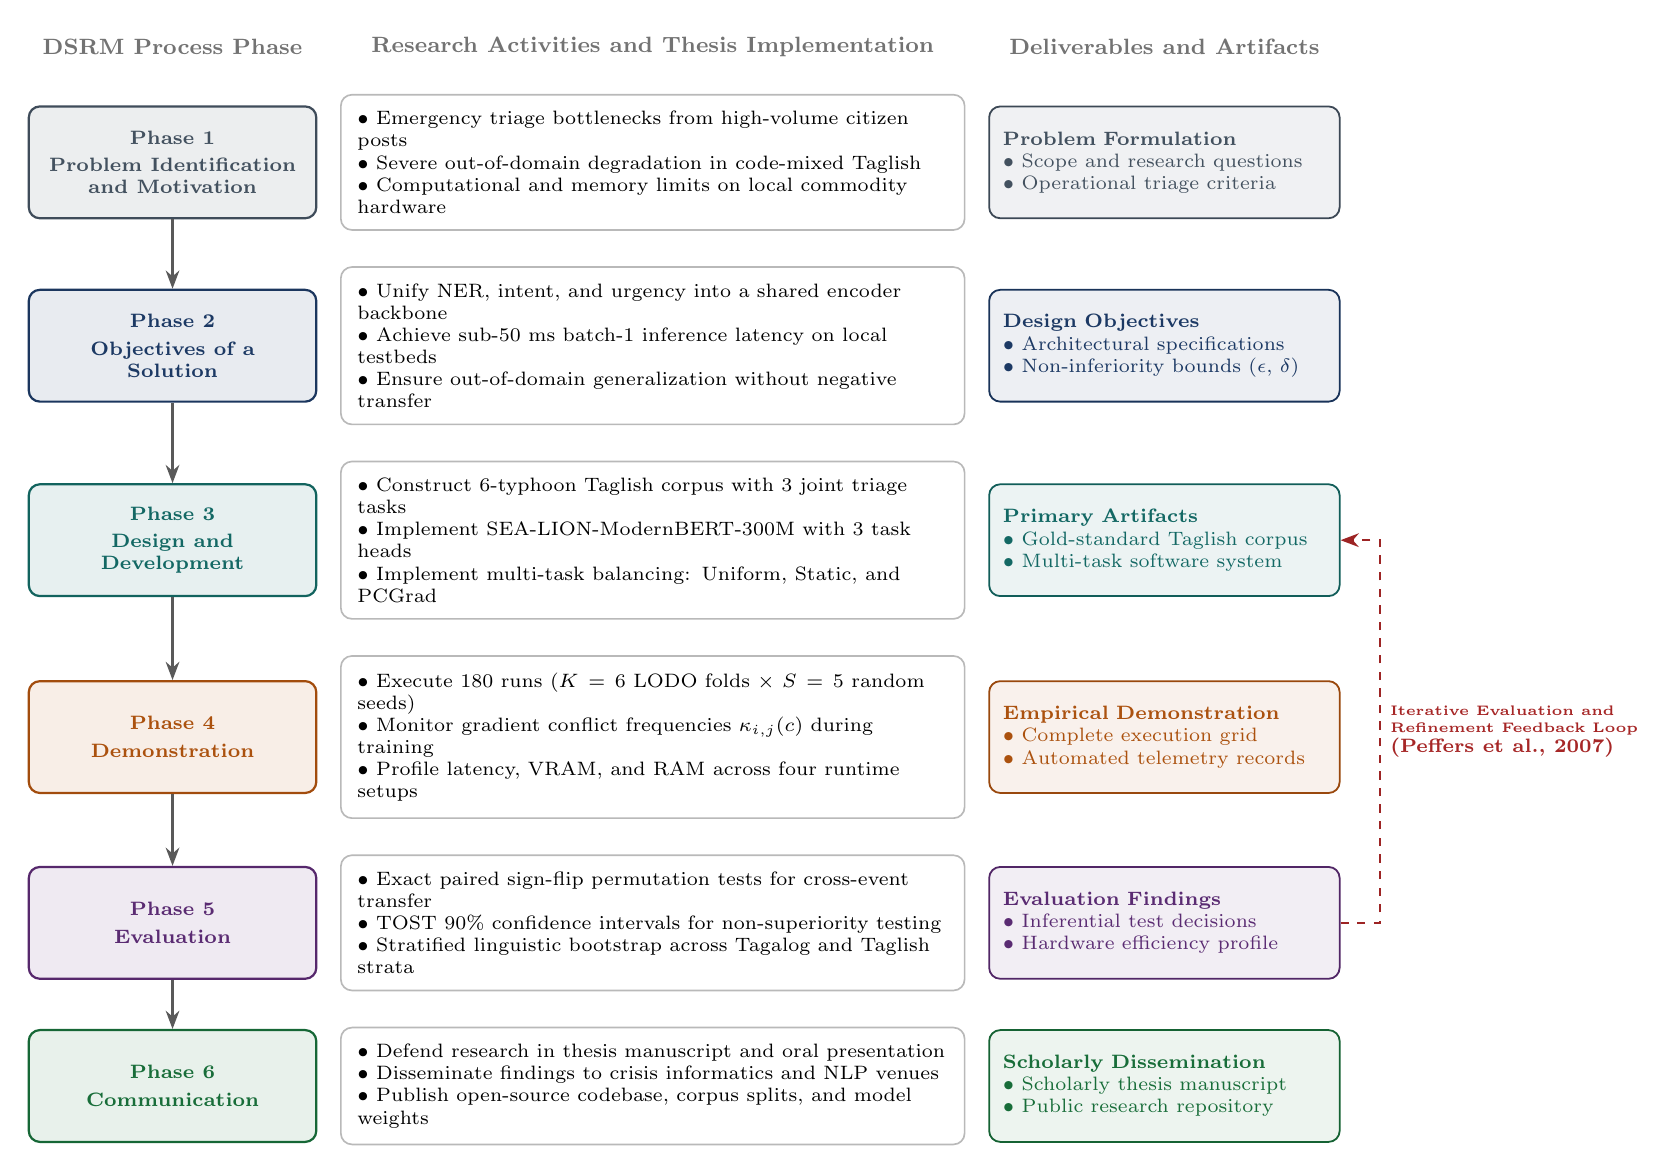
\begin{tikzpicture}[
    font=\small,
    >=Stealth,
    node distance=0.35cm and 0.45cm,
    every node/.append style={execute at begin node={\hyphenpenalty=10000\exhyphenpenalty=10000\relax}},
    % Styles
    badge/.style={
        draw=#1!90!black,
        fill=#1!10,
        rounded corners=4pt,
        align=center,
        inner sep=5pt,
        font=\scriptsize\bfseries,
        line width=0.8pt,
        text=#1!95!black,
        text width=3.3cm,
        minimum height=1.42cm
    },
    activity/.style={
        draw=gray!55,
        fill=white,
        rounded corners=4pt,
        align=left,
        inner sep=6pt,
        font=\scriptsize,
        line width=0.6pt,
        text width=7.5cm,
        minimum height=1.42cm
    },
    artifact/.style={
        draw=#1!85!black,
        fill=#1!8,
        rounded corners=4pt,
        align=left,
        inner sep=5pt,
        font=\scriptsize,
        line width=0.65pt,
        text=#1!95!black,
        text width=4.1cm,
        minimum height=1.42cm
    },
    flowarrow/.style={
        ->,
        thick,
        draw=gray!70!black
    },
    looparrow/.style={
        ->,
        thick,
        dashed,
        draw=crimsonred!90!black
    }
]

    % =========================================================================
    % HEADER ROW
    % =========================================================================
    \node[font=\bfseries\footnotesize, text=gray!90!black, align=center, text width=3.3cm] (h1) 
        {DSRM Process Phase};
    \node[font=\bfseries\footnotesize, text=gray!90!black, align=center, text width=7.5cm, right=0.45cm of h1] (h2) 
        {Research Activities and Thesis Implementation};
    \node[font=\bfseries\footnotesize, text=gray!90!black, align=center, text width=4.1cm, right=0.45cm of h2] (h3) 
        {Deliverables and Artifacts};

    % =========================================================================
    % PHASE 1: Problem Identification
    % =========================================================================
    \node[activity, below=0.35cm of h2] (a1) {
        $\bullet$ Emergency triage bottlenecks from high-volume citizen posts\\
        $\bullet$ Severe out-of-domain degradation in code-mixed Taglish\\
        $\bullet$ Computational and memory limits on local commodity hardware
    };
    \node[badge=slategrey] (b1) at (h1 |- a1) {
        Phase 1\\[2pt]
        Problem Identification\\
        and Motivation
    };
    \node[artifact=slategrey] (o1) at (h3 |- a1) {
        \textbf{Problem Formulation}\\
        $\bullet$ Scope and research questions\\
        $\bullet$ Operational triage criteria
    };

    % =========================================================================
    % PHASE 2: Objectives of a Solution
    % =========================================================================
    \node[activity, below=0.45cm of a1] (a2) {
        $\bullet$ Unify NER, intent, and urgency into a shared encoder backbone\\
        $\bullet$ Achieve sub-50 ms batch-1 inference latency on local testbeds\\
        $\bullet$ Ensure out-of-domain generalization without negative transfer
    };
    \node[badge=navyblue] (b2) at (h1 |- a2) {
        Phase 2\\[2pt]
        Objectives of a\\
        Solution
    };
    \node[artifact=navyblue] (o2) at (h3 |- a2) {
        \textbf{Design Objectives}\\
        $\bullet$ Architectural specifications\\
        $\bullet$ Non-inferiority bounds ($\epsilon$, $\delta$)
    };

    % =========================================================================
    % PHASE 3: Design & Development
    % =========================================================================
    \node[activity, below=0.45cm of a2] (a3) {
        $\bullet$ Construct 6-typhoon Taglish corpus with 3 joint triage tasks\\
        $\bullet$ Implement SEA-LION-ModernBERT-300M with 3 task heads\\
        $\bullet$ Implement multi-task balancing: Uniform, Static, and PCGrad
    };
    \node[badge=tealblue] (b3) at (h1 |- a3) {
        Phase 3\\[2pt]
        Design and\\
        Development
    };
    \node[artifact=tealblue] (o3) at (h3 |- a3) {
        \textbf{Primary Artifacts}\\
        $\bullet$ Gold-standard Taglish corpus\\
        $\bullet$ Multi-task software system
    };

    % =========================================================================
    % PHASE 4: Demonstration
    % =========================================================================
    \node[activity, below=0.45cm of a3] (a4) {
        $\bullet$ Execute 180 runs ($K=6$ LODO folds $\times$ $S=5$ random seeds)\\
        $\bullet$ Monitor gradient conflict frequencies $\kappa_{i,j}(c)$ during training\\
        $\bullet$ Profile latency, VRAM, and RAM across four runtime setups
    };
    \node[badge=ambergold] (b4) at (h1 |- a4) {
        Phase 4\\[2pt]
        Demonstration
    };
    \node[artifact=ambergold] (o4) at (h3 |- a4) {
        \textbf{Empirical Demonstration}\\
        $\bullet$ Complete execution grid\\
        $\bullet$ Automated telemetry records
    };

    % =========================================================================
    % PHASE 5: Evaluation
    % =========================================================================
    \node[activity, below=0.45cm of a4] (a5) {
        $\bullet$ Exact paired sign-flip permutation tests for cross-event transfer\\
        $\bullet$ TOST 90\% confidence intervals for non-superiority testing\\
        $\bullet$ Stratified linguistic bootstrap across Tagalog and Taglish strata
    };
    \node[badge=purplecat] (b5) at (h1 |- a5) {
        Phase 5\\[2pt]
        Evaluation
    };
    \node[artifact=purplecat] (o5) at (h3 |- a5) {
        \textbf{Evaluation Findings}\\
        $\bullet$ Inferential test decisions\\
        $\bullet$ Hardware efficiency profile
    };

    % =========================================================================
    % PHASE 6: Communication
    % =========================================================================
    \node[activity, below=0.45cm of a5] (a6) {
        $\bullet$ Defend research in thesis manuscript and oral presentation\\
        $\bullet$ Disseminate findings to crisis informatics and NLP venues\\
        $\bullet$ Publish open-source codebase, corpus splits, and model weights
    };
    \node[badge=forestgreen] (b6) at (h1 |- a6) {
        Phase 6\\[2pt]
        Communication
    };
    \node[artifact=forestgreen] (o6) at (h3 |- a6) {
        \textbf{Scholarly Dissemination}\\
        $\bullet$ Scholarly thesis manuscript\\
        $\bullet$ Public research repository
    };

    % =========================================================================
    % CONNECTING ARROWS (Between Badges)
    % =========================================================================
    \draw[flowarrow] (b1) -- (b2);
    \draw[flowarrow] (b2) -- (b3);
    \draw[flowarrow] (b3) -- (b4);
    \draw[flowarrow] (b4) -- (b5);
    \draw[flowarrow] (b5) -- (b6);

    % =========================================================================
    % ITERATIVE DSRM FEEDBACK LOOP (Phase 5 to Phase 3)
    % =========================================================================
    \draw[looparrow] (o5.east) -- ++(0.5, 0) |- 
        node[pos=0.25, right, font=\tiny\bfseries, text=crimsonred!95!black, align=left] {
            Iterative Evaluation and\\
            Refinement Feedback Loop\\
            \scriptsize (Peffers et al., 2007)
        } 
        (o3.east);

\end{tikzpicture}
\end{document}
